
\chapter{Techniques for Protocol Optimization}\label{sec:Techniques}

Optimizing secure function evaluation to make it more practical for
real world use will be the focus of this thesis.  Traditional methods
for SFE, such as Yao's secure circuit evaluation protocol \cite{Yao86},
are many orders of magnitude slower than the straightforward insecure evaluation of
functions, with factors of thousands or more.  Asymtotically, the time
required to perform secure function evaluation
is equivalent to the time required to execute the function itself.
For example, the Yao protocol
requires time and communication linear in the number of circuit gates.
However, the need to encrypt every gate with multiple keys, and to
perform oblivious transfer on every circuit input is the cause of the enormous
slowdowns.  These tremendous performance penalties in the generic constructions highlight
the need for optimizing SFE.

There are various ways to approach the problem of designing optimized
secure function evaluation protocols.  This thesis focuses
on three general methodologies. From most specific to most general,
three approaches we have looked at are algorithm specific, algorithm
\emph{class} specific, and a general approach that is applicable to
all computable functions. The trade-off between these different approaches
is a balance between performance and general applicability. This trade-off
has an analogy in the literature of programming language compiler
optimizations. General code optimizations, such as loop-unrolling
or strength-reduction can make all code faster to a limited degree
(although this is not guaranteed), but tuning a specific algorithm
by hand often yields superior results. Algorithm class methods fall
in between, with conceptual ideas that apply to classes of algorithms
related by design methodology, such as dynamic programming problems.


\section{General: Protocol Optimization using Ordered Binary Decision Diagrams}
\label{OBDD-section}

In this work, we evaluated the use of alternate representation of
Boolean circuits as a way to create more efficient general purpose
secure function evaluation protocols. An \emph{Ordered Binary Decision
Diagram} (OBDD) is a directed acyclic graph-based representation of
a Boolean function that has been used in a variety of applications
in computer-aided design, including symbolic model checking (a technique
for verifying designs), verification of combinational logic, and verification
of finite-state concurrent systems \cite{Bryant:BDD,Clarke:book}.
OBDDs can be readily extended to represent functions with arbitrary
domains and ranges. An OBDD is similar to a decision tree, in that
evaluation is performed from a head node to leaves. However, an OBDD
is not ordinarily a tree, because internal nodes with identical structure
are shared. Given a function $f(x_{1},x_{2},\cdots,x_{n})$, the OBDD
for that function will have $n$ levels, with the $i^{th}$ level
corresponding to variable $x_{l_{i}}$, where $(l_{1},\cdots,l_{n})$
is a permutation of $(1,\cdots,n)$. There is a unique canonical OBDD
corresponding to any function with respect to a given ordering $(l_{1},\cdots,l_{n})$.
An example of an OBDD to compute the function $F(x)=\#x1\#x3>\#x2\#x4$
(two-bit millionaires' problem) is shown in \ref{fig:OBDD-example}.

%
\begin{figure}
\begin{centering}
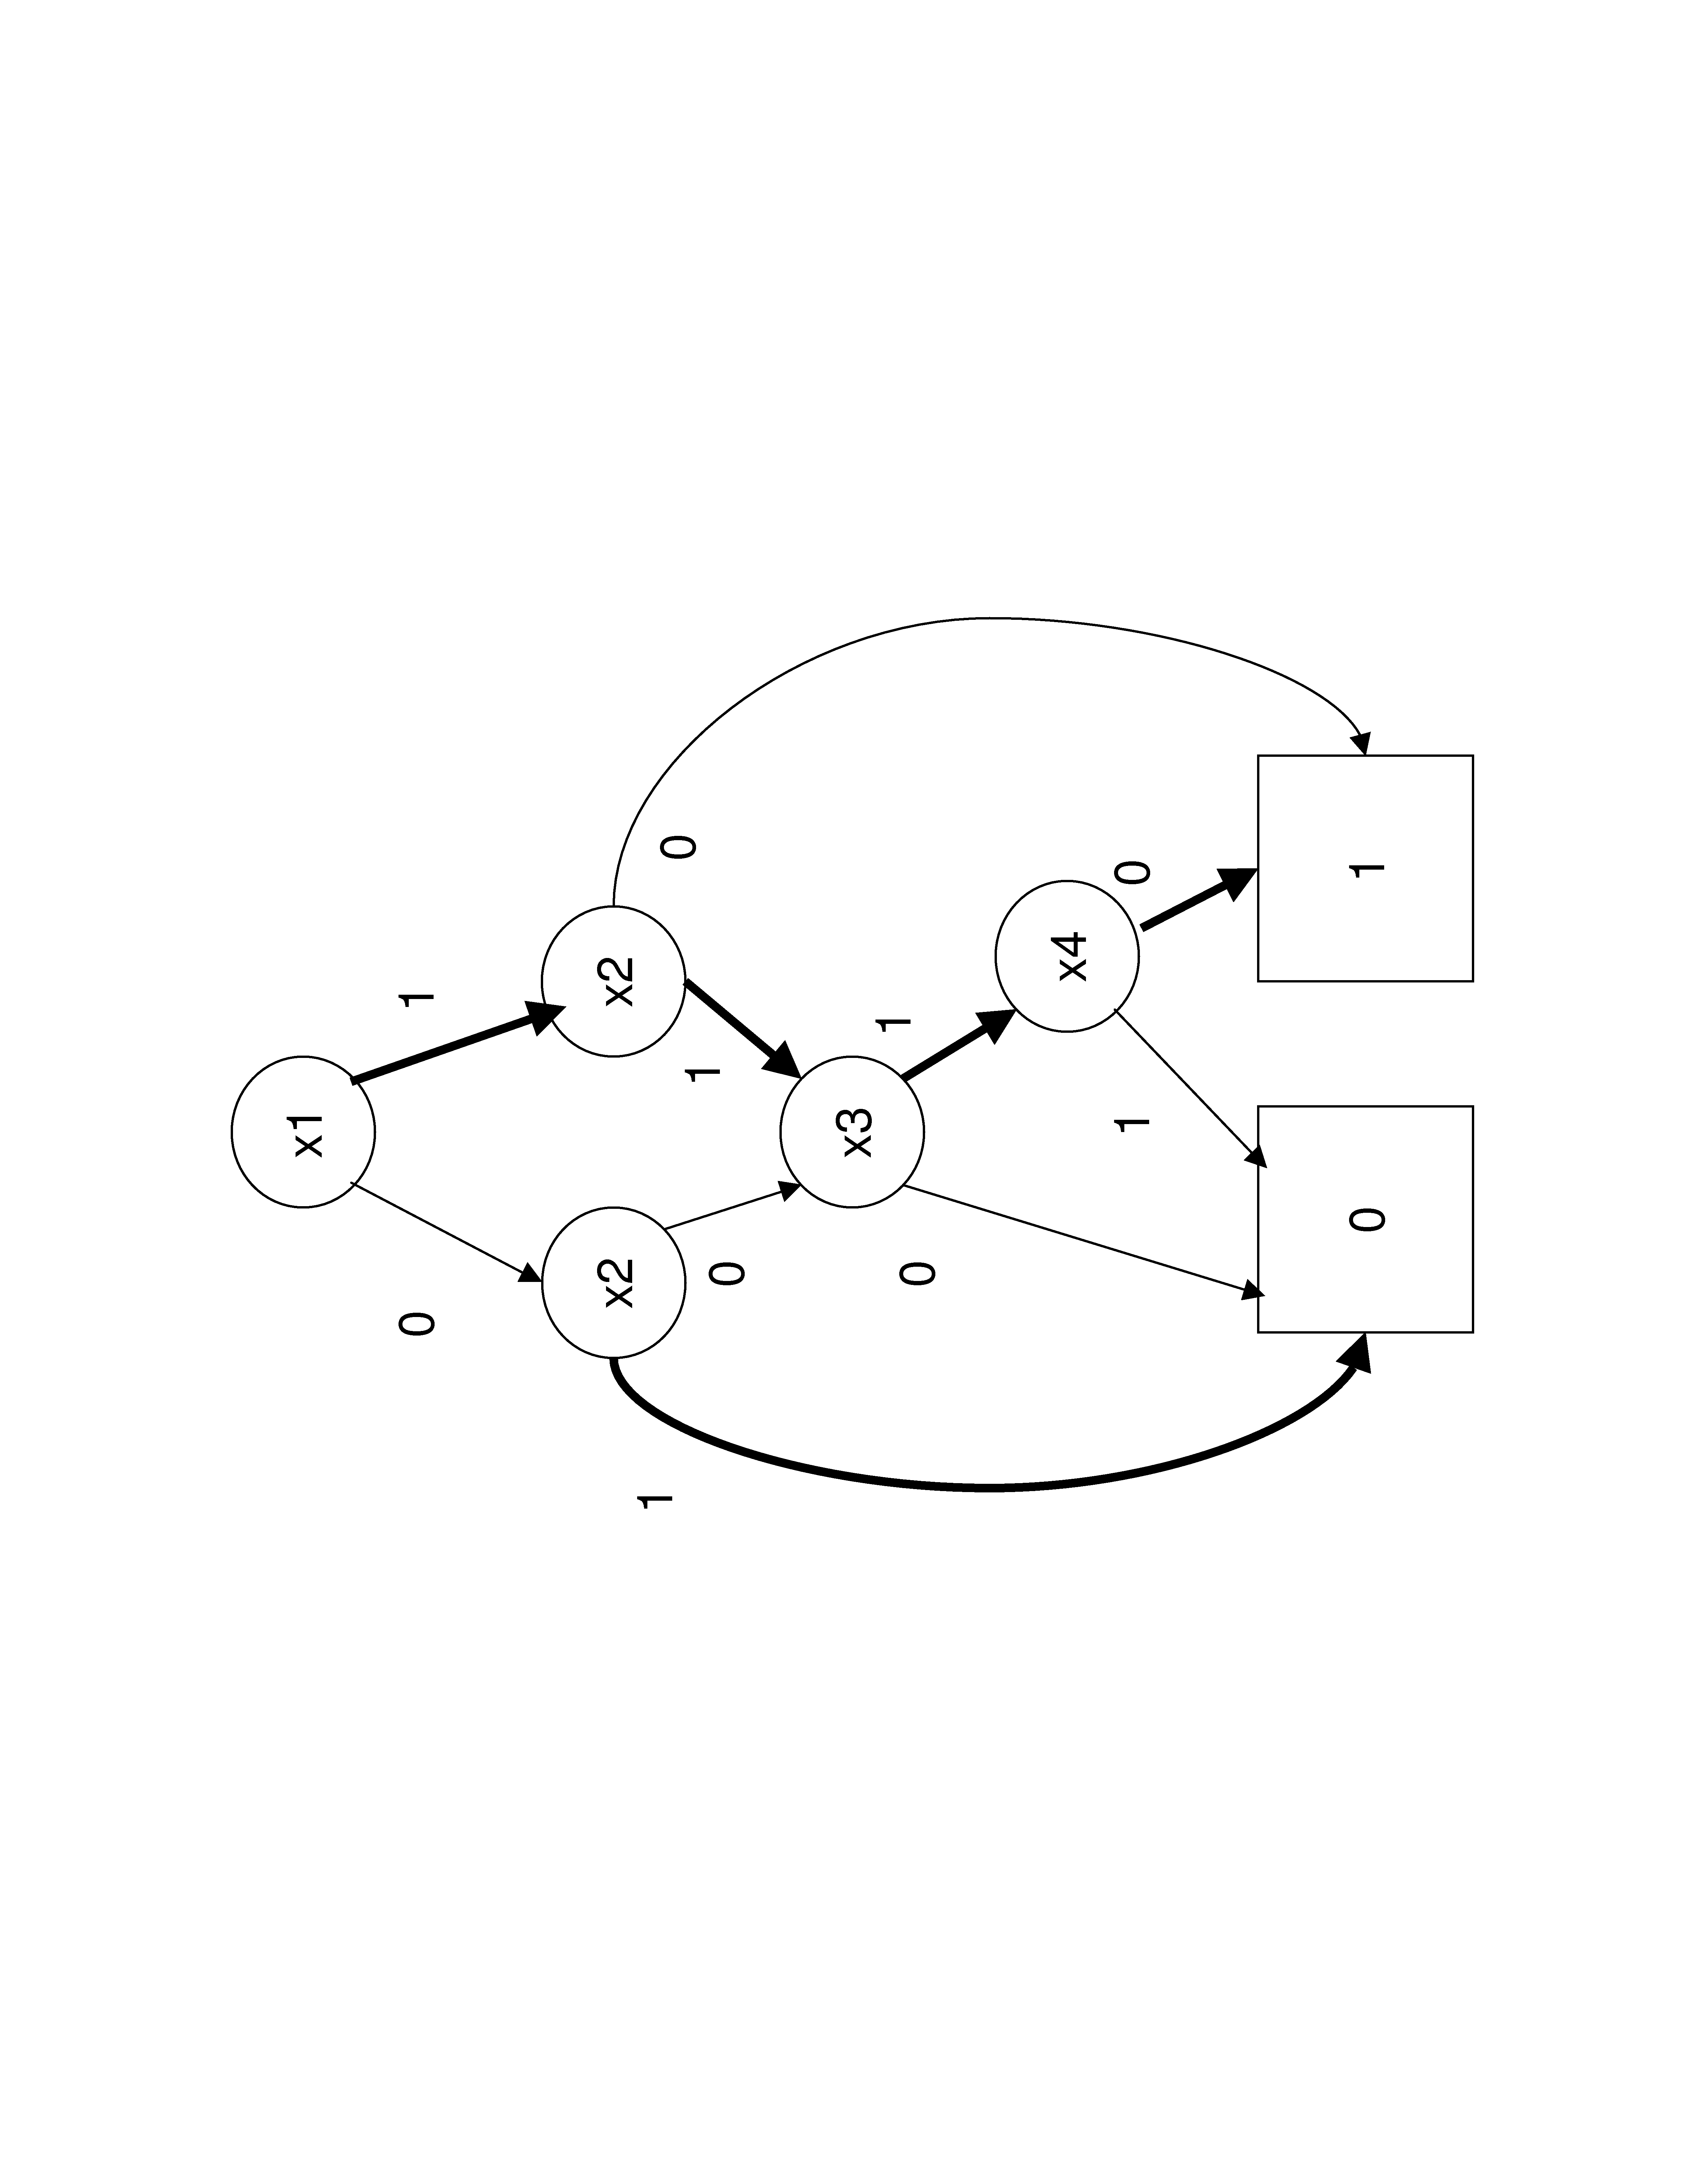
\includegraphics[scale=0.4,angle=270]{obdd1}
\par\end{centering}

\caption{\label{fig:OBDD-example}OBDD for two-bit millionaires' problem}

\end{figure}


In \cite{kruger06}, we presented an SFE protocol that directly uses
an OBDD representation of the function $f$ to be jointly computed.
The advantage of using an OBDD representation over the Boolean gate-representation
is that OBDDs are more succinct for certain classes of functions than
the Boolean gate representation, including most linear functions.
For example, the OBDD representation is more efficient than the Boolean
gate representation for 8-bit AND, 8-bit addition, and the millionaires'
and billionaires' problems \cite{Yao86} OBDDs are not a universal
solution, however, for other functions, such as multiplication, the
OBDD can be far worse than the Boolean gate representation, due to
exponential node explosion \cite{Bryant:BDD}. For the classes of
functions in which the OBDD representation is efficient, our thesis
\cite{kruger06} shows that the protocol described next can perform
2 to 4 times better than the classical Yao protocol.

The protocol is loosely designed in a similar fashion as Yao's protocol
\cite{Yao86}. We present two variations of the protocol. An overview
of the 3 main steps of the protocols are shown in figure \ref{fig:OBDD-overview},
using the example millionaires' problem pictured above. In the first
step, Alice sends to Bob the encrypted OBDD. The next step is Bob
acquiring a subset of the encryption keys from Alice using $OT_{2}^{1}$.
In the final step, Bob uses the obtained keys to decrypt a single
path through the OBDD yielding the result of the computation. A formal
description follows. 

%
\begin{figure}
\begin{centering}
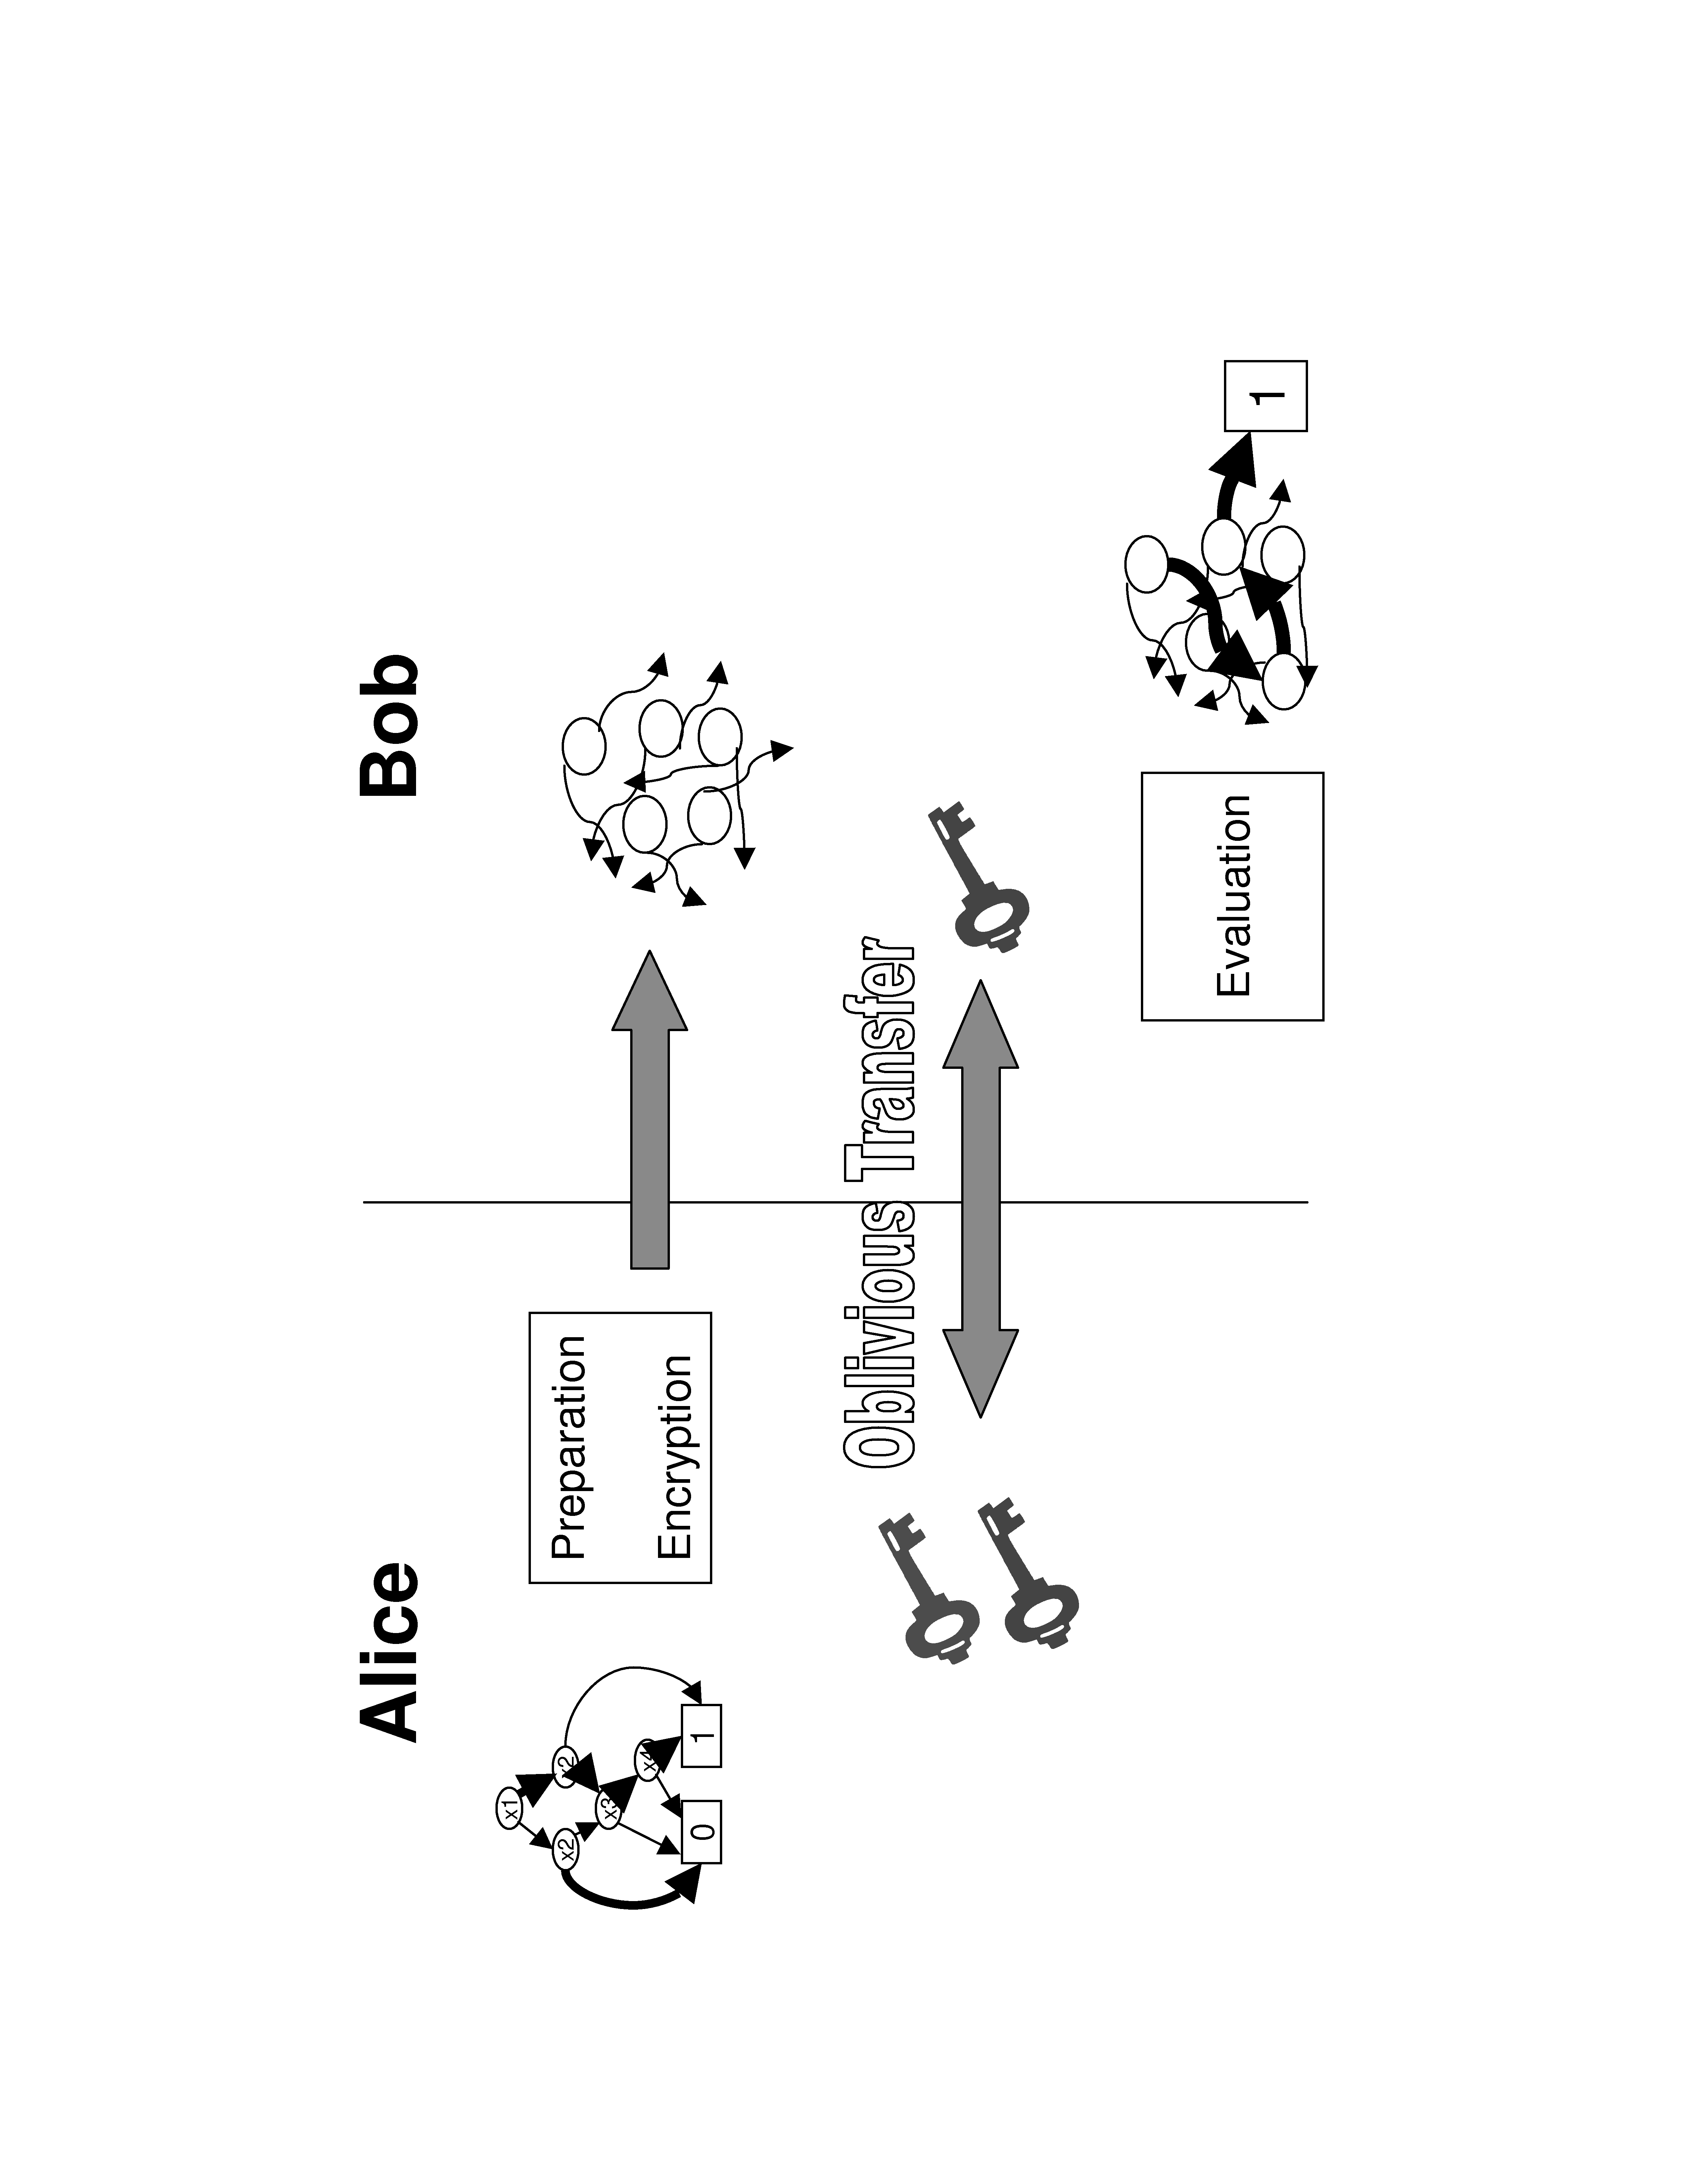
\includegraphics[scale=0.4,angle=270]{obdd_proto_overview}
\par\end{centering}

\caption{\label{fig:OBDD-overview}OBDD secure evaluation protocol}

\end{figure}


%\begin{flushleft}
Assume that both parties' inputs include the $OBDD(f)$ for the Boolean
function $f(x_{1},x_{2},\cdots,x_{n})$ with the ordering $x_{1}<x_{2}<\cdots<x_{n}$.
Furthermore, Alice holds the inputs $(i_{1},\ldots,i_{k})$ corresponding
to the first $k$ variables $x_{1},\ldots,x_{k}$, and Bob has the
inputs $(i_{k+1},\ldots,i_{n})$.
\par\end{flushleft}
\begin{enumerate}
\item Alice performs the following steps: 

\begin{enumerate}
\item She traverses the $OBDD(f)$ using her input $(i_{1},\cdots,i_{k})$,
which results in a node $v_{init}$ at level $k$.
\item She uniformly and independently at random creates $(n-k)$ pairs of
secrets $(s_{1}^{0},s_{1}^{1}),\cdots,(s_{n-k}^{0},s_{n-k}^{1})$.
In addition, for each node $v$ in the $OBDD(f)$ whose level is between
$k$ and $n-1$, Alice also creates a secret $s_{v}$.
\item She assigns a uniformly random label to each node whose level is between
$k$ and $n$. We refer to the randomly assigned label of node $v$
using the notation $label(v)$.
\item Next, Alice augments $OBDD(f)$ with some number of dummy nodes (to
ensure that Bob always traverses $n-k$ nodes in his phase of the
protocol).
\item Alice garbles all nodes whose level is between $k$ and $n-1$ in
the following manner. Let $v$ be a node in $OBDD(f)$ such $k\leq{\it level}(v)\leq n-1$
and define ${\it level}(v)=\ell$. The encryption of node $v$, denoted
by $E^{(v)}$, is a label and a randomly ordered ciphertext pair \[
\left(label(v)\,\,,\,\, E_{s_{v}\oplus s_{\ell-k+1}^{0}}(label(low(v))\,\|\, s_{{\it low}(v)})\,\,\,,\,\,\, E_{s_{v}\oplus s_{\ell-k+1}^{1}}(label(high(v))\,\|\, s_{{\it high}(v)})\right)\,\,\,,\]
 where the labels are pre-pended to the secret with a separator symbol
and the order of the ciphertexts is determined by a fair coin flip.
Roughly speaking, the secrets corresponding to the $0$-successor
and $1$-successor of node $v$ are encrypted with the secret corresponding
to $v$ and its level.


Note that dummy nodes have the same structure as normal nodes, except
that the ciphertext pair contain encryptions of the same message since
dummy nodes have the same $0$ and $1$-successors. Provided the encryption
scheme is semantically secure, this poses no problem since the keys
are chosen uniformly at random.

Lastly, there are two terminal nodes of the form $(b,label(t_{b}))$
for $b=0$ or $1$. Recall that $OBDD(f)$ has two terminal nodes,
denoted as $0$ and $1$, that are at level $n$.

\item Once Alice is done encrypting, she sends to Bob the encryption of
all nodes whose level is between $k$ and $n$ and the secret $s_{v_{init}}$
corresponding to node $v_{init}$ at level $k$. We called this the
garbled OBDD.
\end{enumerate}
\item Bob performs the following steps: 

\begin{enumerate}
\item He engages in $n-k$ 1-out-of-2 oblivious transfers to obtain the
secrets corresponding to his input. For example, if his input $i_{j}$
is $0$, then he obtains the (level) secret $s_{j-k}^{0}$; otherwise,
he obtains the secret $s_{j-k}^{1}$.
\item Now Bob is ready to start his computation. Suppose $i_{k+1}=0$. With
$s_{1}^{0}$ and $s_{v_{init}}$, he decrypts both ciphertexts in
$E^{(v_{init})}$ and decides which gives the correct result by using
the verifiable range property of the encryption scheme. Bob now has
both $s_{{\it low}(v)}$ (the secret corresponding to the $0$-successor
of $v_{init}$) and $label(low(v))$ (which tells Bob which encrypted
node is used to evaluate his next input). Continuing this way, Bob
eventually obtains a label corresponding to one of the terminal nodes,
which determines the result of the OBDD on the shared inputs. Bob
sends this result to Alice. 
\end{enumerate}
\end{enumerate}



We then define an optimized variation which is identical to the protocol
just described, except that Alice first reduces the number of nodes
to be sent to Bob using an operation called \emph{restriction}, which
is a partial evaluation applied to OBDDs. Restriction is defined as
follows. 

Given an $n$ variable Boolean function $f(x_{1},x_{2},\cdots,x_{n})$
and a Boolean value $b$, the restriction $f\mid_{x_{i}\leftarrow b}$
is a Boolean function of $n-1$ variables $x_{1},\cdots,x_{i-1},x_{i+1},\cdots,x_{n}$.
$f\mid_{x_{i}\leftarrow b}(x_{1},\cdots,x_{i-1},x_{i+1},\cdots,x_{n})$
is equal to $f(x_{1},\cdots,x_{i-1},b,x_{i+1},\cdots,x_{n})$. Essentially,
$f\mid_{x_{i}\leftarrow b}$ is the function obtained by substituting
the value $b$ for the variable $x_{i}$ in the function $f$. The
restriction operation can be performed over multiple variables by
restricting each variable independently, e.g., $f\mid_{x_{i}\leftarrow b,x_{j}\leftarrow b'}=(f\mid_{x_{i}\leftarrow b})\mid_{x_{j}\leftarrow b'}$.
The order in which the variables are restricted is unimportant.

\begin{flushleft}
For protocol 2, both parties' inputs include the $OBDD(f)$ for the
Boolean function $f(x_{1},x_{2},\cdots,x_{n})$ with the ordering
$x_{1}<x_{2}<\cdots<x_{n}$. Furthermore, Alice holds the inputs for
the variables in the set $X_{A}$ and Bob holds the inputs for the
variables in the set $X_{B}\;=\;\{x_{1},\cdots,x_{n}\}-X_{A}$. 
\par\end{flushleft}
\begin{enumerate}
\item Alice performs the following steps: 

\begin{enumerate}
\item Alice computes the OBDD ${\cal O}_{A}$ as the restriction of her
inputs on the function $f\mid_{X_{A}}$. 
\item Alice encrypts the $O_{A}$ and sends it to Bob. This step is exactly
the same as in for Protocol 1. Alice also sends the secret corresponding
to the root of the OBDD ${\cal O}_{A}$.
\end{enumerate}
\item The computation for Bob is exactly the same as that for Protocol 1.
\end{enumerate}
The results of this work demonstrated that OBDDs showed improved performance
with secure evaluation of certain functions. 

\section{Problem Specific: Protocol Optimization of Evaluating Hash Functions for Password Authentication}
In chapter \ref{chapter:pw}, 
%based on our paper Secure Password Authentication Using SFE \cite{Kruger10}, 
we use some properties of the problem of
authentication to transform the semi-honest protocol into an efficient protocol that is secure in the malicious model.  
This protocol takes
advantage of specific properties of the authentication problem and takes "shortcuts" to achieve efficiency.  Although
these shortcuts would not be secure in a general SFE setting, we prove that these shortcuts are in fact secure in the 
context of the authentication protocol presented.  This allows us to design a protocol in which a malicious adversary
is thwarted with probability $1-2^{-l}$ where $l$ is a security parameter representing the number of semi-honest circuits.
We show that on modern multicore processors, the authentication can be performed in a matter of seconds, which we believe is practical
for interactive use between servers and authenticating users.

\section{Class of Algorithm Specific: Protocol Optimization of Dynamic Programming}

In this work, we considered a design \emph{methodology} for creating
secure protocols based on typical dynamic programming algorithms.
Unlike the OBDD protocol discussed in the previous section, this is
not an automatic tool for generating secure protocols, but rather
a set of concepts that are applicable to designing secure protocols
for evaluation dynamic programming algorithms. We illustrate these
ideas with several example protocols for computing the edit distance
problem, which is the minimum number of character insertions, deletions,
and substitutions needed to change string $x$ to string $y$.

Let ${\cal P}(x,y)$ be a problem with two inputs $x$ and $y$. Typically,
a dynamic-programming algorithm ${\cal A}_{{\cal P}}$ for problem
${\cal P}$ has the following components:
\begin{itemize}
\item A set $S$ of sub-problems and a dependency relation $R\subseteq S\times S$
between the sub-problems. Intuitively, $(s,s')\in R$ means that the
sub-problem $s'$ depends on the sub-problem $s$. If there is a dependency
between $s$ and $s'$, we write it as $s\rightarrow s'$. In the
case of the problem of computing edit-distance between two strings
$\alpha$ and $\beta$ of length $n$ and $m$, the set of sub-problems
is $[0,\cdots,n]\times[0,\cdots,m]$. For all sub-problems $(i,j)$
such that $i\not=0$ and $j\not=0$, we have the following dependencies:
$(i-1,j)\rightarrow(i,j)$, $(i,j-1)\rightarrow(i,j)$, and $(i-1,j-1)\rightarrow(i,j)$.
The \textit{base sub-problems} are $s\in S$ such that they have no
dependencies. For the edit-distance problem, the base sub-problems
are: \[
\begin{array}{l}
\{(i,0)\;\mid\;0\leq i\leq n\}\\
\{(0,j)\;\mid\;0\leq j\leq m\}\end{array}\]
 We also assume that there is a unique root sub-problem ${\it root}\in S$
such that there does not exist a sub-problem that depends on ${\it root}$.
For the edit-distance problem the unique root sub-problem is $(n,m)$.
\item Each sub-problem $s$ is assigned a value ${\it val}(s)$. The goal
is to compute ${\it val}({\it root})$. The function ${\it val}$
from $S$ to $\Re$ assigns values to sub-problems, such that it satisfies
the following properties:

\begin{itemize}
\item For all the base sub-problems $s\in S$, ${\it val}(s)$ is defined.
\item Let $s\in S$ be a non-base sub-problem. Define ${\it pred}(s)$ as
all the predecessors of $s$, i.e. the set ${\it pred}(s)$ is defined
as $\{s'\;\mid\; s'\rightarrow s\}$. Assume that ${\it pred}(s)$
is equal to $\{s_{1},\cdots,s_{k}\}$. There is a recursive function
$f$ defining ${\it val}(s)$ in terms of ${\it val}(s_{1}),{\it val}(s_{2}),\cdots,{\it val}(s_{k})$,
$s(x)$, and $s(y)$, where $s(x)$ and $s(y)$ are parts of the input
$x$ and $y$ that are relevant to the sub-problem $s$. In case of
the edit-distance problem ${\it val}((i,j))$ is equal to $D(i,j)$. 
\end{itemize}
\end{itemize}
We implemented three variations of the protocol in \cite{kruger07},
and showed that the techniques produce efficient ways to compute the
edit distance of two strings. For example, the protocol is able to
compute the edit distance of two strings of length $200$ (which has
$200^{2}=40000$ sub-computations), in under 10 minutes. Our most
efficient protocol computes elements of the dynamic programming matrix
in large blocks during each round of the computation. We experimentally
determined than a block size of $(20,20)$ yielded an optimum trade-off
between a decreased number of rounds, and larger block circuits. Using
a $(20,20)$ circuit allows $20^{2}=400$ elements of the matrix to
be evaluated during each round of the protocol, which allows the overall
$(200,200)$ problem to be evaluated in $100$ rounds. In comparison,
using the generic techniques to compile the edit distance algorithms
into a secure circuit produced circuits which were to too large for
evaluation beyond problems of size $(25,25)$.


\section{Algorithm Specific: Protocol Optimization of K-Means Clustering}

The $k$-means algorithm is a common clustering technique in data
mining. Suppose that we are given $n$ samples $x_{1},\cdots,x_{n}$,
where each sample is a $m$-dimensional vector of real numbers. The
problem is to assign the samples to $c$ clusters such a manner that
similar points are grouped together. Similarity is defined using a
distance metric. The standard clustering algorithm maintains $c$
means $\mu_{1},\cdots,\mu_{c}$. Initially, assume that the means
are assigned arbitrary values. A sample $x_{i}$ is deemed to be in
the cluster $j$ if it is closest to the mean $\mu_{j}$, where mean
of a cluster $\{x'_{1},\cdots,x'_{r}\}$ is $\frac{x'_{1}+\cdots,x'_{r}}{r}$.
In a Euclidean space, the distance between two $m$-dimensional vectors
$x$ and $y$ is $\sum_{j=1}^{m}(x[j]-y[j])^{2}$, where $x[j]$ is
the $j$-th element of the vector $x$. Other distance metrics~\cite[Chapter 10]{pattern-classification},
such as scatter metrics, can be used instead of the distance metric
mentioned above. Each iteration of the $k$-means algorithms recomputes
the means and reclassifies the samples. The algorithm terminates when
it detects no change in the means. See \ref{fig:clusters} for an
illustration.

%
\begin{figure}
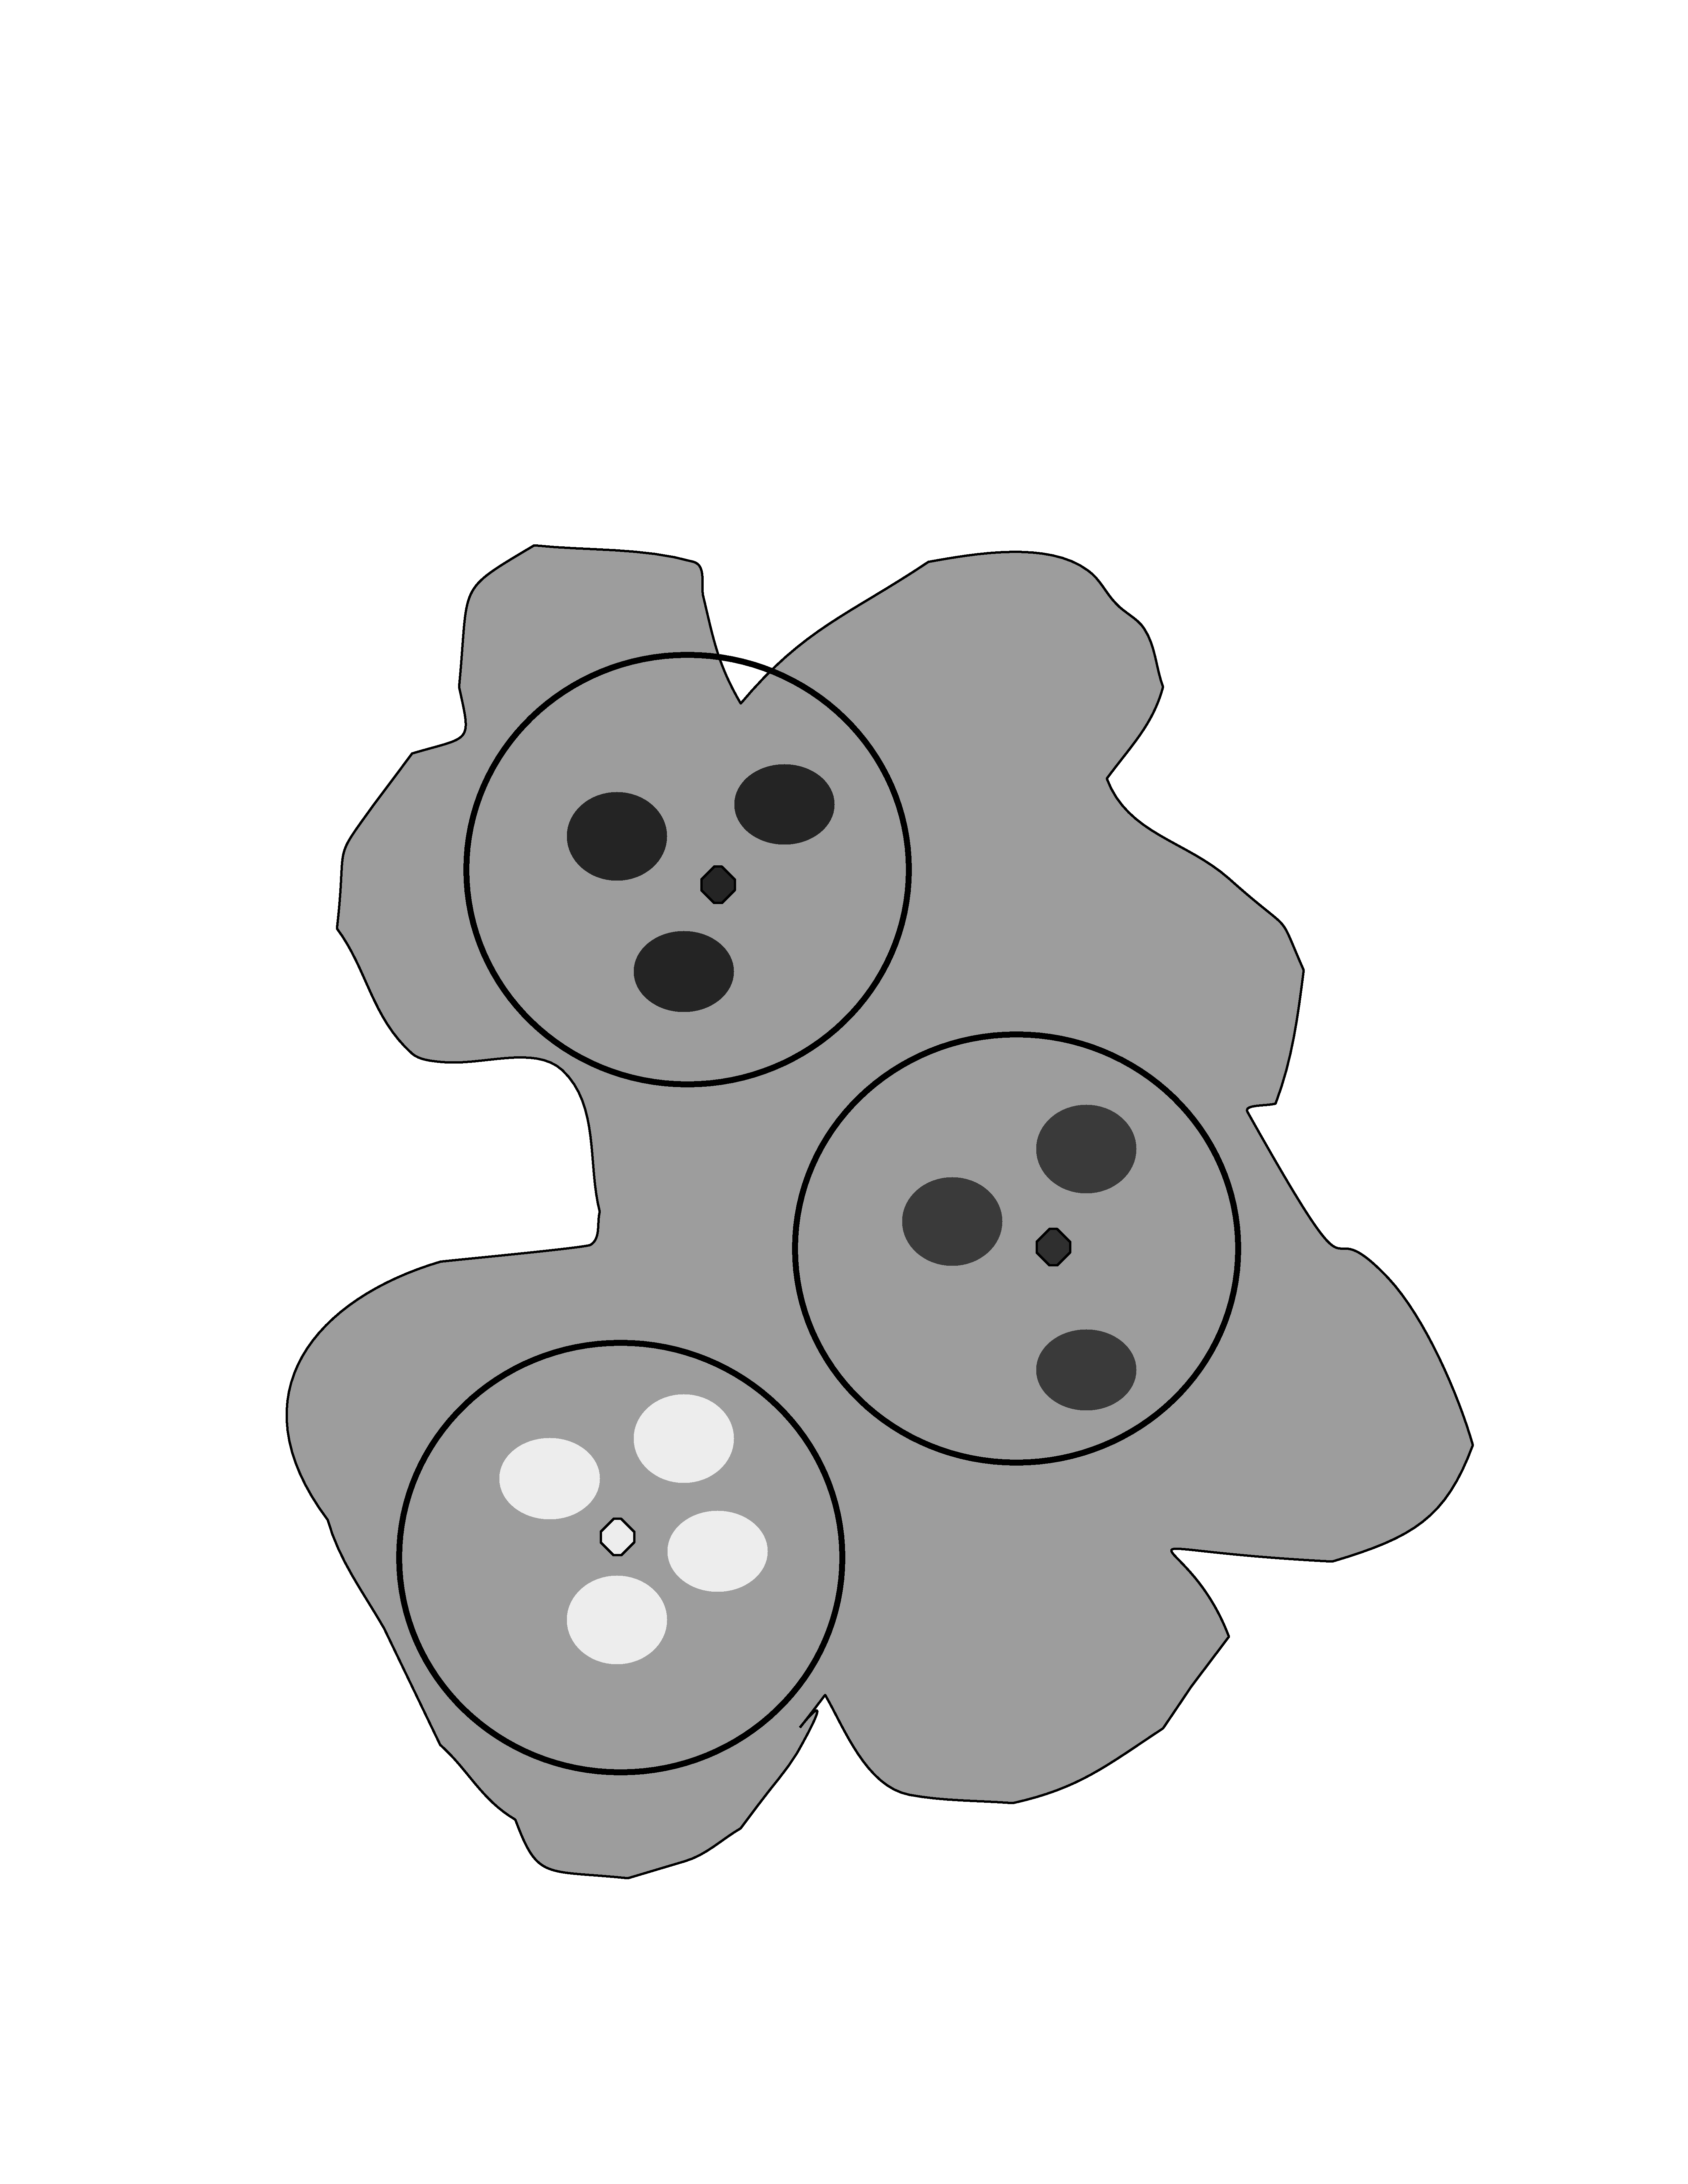
\includegraphics[scale=0.3,angle=270]{clusters}

\caption{\label{fig:clusters}Thirteen data points after clustering. The small
dots are cluster means.}

\end{figure}


We implemented protocols to securely evaluate this algorithm in \cite{kruger05},
and showed that a protocol based on homomorphic encryption was able
to classify partitioned data sets with tens of thousands of data points
in under two minutes, which is about 15 times slower than the protocol
implemented in a straightforward way without privacy protection, and
over 100 times faster than the same protocol built with Yao circuits.


\section{Other Optimizations}\label{sub:Other-Optimizations}

In the usual formulation of secure function evaluation, there are
designated outputs for each party, and it is required that no extra
information is learned by any party. This definition could be expanded
to assign non-output values the labels {}``sensitive'' and {}``non-sensitive'',
where the protocol is considered secure if no sensitive information
is leaked. Since the overhead of privacy protection is substantial,
I propose to research the of design secure protocols that use this
relaxation of the problem definition to improve efficiency. 

In section \ref{sub:Primitives}, I presented many basic cryptographic
primitives that are used in SFE. Improving the state of the art of
any one of those primitives would automatically benefit all SFE protocols
that make use of that primitive. Based on my experience with real
implementations of SFE protocols, the oblivious transfer steps tend
to be very expensive in terms of space and communication. Common oblivious
transfer protocols are based on discrete logarithms, but other trapdoor
functions may be used as well. One thing I propose to try is implementing
Naor-Pinkas \cite{Noar-Pinkas:2001} using more compact representations,
for example, with elliptic curve groups. I have recently developed
a new $OT_{2}^{1}$ protocol, presented in section \ref{sec:OT-SquareRoots}.
I also propose to prove its security and compare its performance with
the Naor-Pinkas protocol. In particular, I conjecture that this protocol
may require less communication overhead than other OT protocols.


\section{An Efficient Protocol Design Framework}\label{sub:An-Efficient-Framework}

Even with all these optimizations, protocols still must be hand-coded.
Each protocol I have implemented has required brand new code to be
written, with only some common cryptographic primitives being shared
between implementations. In this case, I define the term protocol
to mean a structured sequence of communications between parties which
enables the computation to performed. Fairplay \cite{Fairplay} suggested
the idea of having a common framework for protocol design, but because
Fairplay is a straightforward implementation of Yao's garbled circuit
method \cite{Yao86}, it suffers from poor performance. Fairplay's
contribution is to create a compiler for expressing algorithms functionally,
and compiling them into a circuit representation suitable for secure
evaluation. In this sense, it functions as a simple CAD design tool.

I propose to take this concept much further, and create an \emph{optimizing}
protocol compiler, aggregating the techniques discussed here, and
creating a tool to greatly simplify the creation of efficient secure
protocols for SFE. The compiler will include the following components:
\begin{itemize}
\item Convenient programming language for expressing secure computations

\begin{itemize}
\item Language will include support as language primitives for common SFE
and cryptographic techniques, such as homomorphic encryption
\item Language will support metadata for designating inputs and outputs
from specific parties, and for classifying the required privacy of
intermediate computations
\end{itemize}
\item Compiler which translates this language into an abstract securely
evaluable {}``machine code'', which consists of securely evaluable
representations of the program.
\item An automated optimizer. The optimizer will automatically try different
representations of the functions, including OBDDs, Boolean circuits,
and other ideas from my research, and search for the most efficient
representation as possible.
\item Manual optimization tools, making it convenient to apply and design
techniques that I have researched. This includes a toolkit of cryptographic
protocols, such as oblivious transfer, which can be used in a black
box way.
\item An embeddable protocol evaluator library, which will allow ordinary
application to make straightforward use of secure function evaluation.
\end{itemize}
The security of protocols produced by the compiler is based on the
security of each individual component of the protocol. For example,
when choosing optimal circuit representations, the compiler will choose
among several possible representations, each of which has a corresponding
secure evaluation protocol. In cases where a computation is broken
into multiple sub-protocols, I will prove that composition of these
sub-protocols maintains the overall security of the protocol.

%
\begin{comment}
\bibliographystyle{plain}
\bibliography{somesh}

\end{comment}
{}
